% $Id: TimeMgr_obj1.tex,v 1.4 2003/08/12 14:32:50 cdeluca Exp $

\subsection{Object Model}

The core Time Manager Library consists of six object-oriented classes (types)
organized in four layers of inheritance, aggregation and composition,
as shown in Figure 1 below.  The primary classes intended for
direct model use are:

\begin{itemize}
\item {\tt ESMF\_TimeInterval}
\item {\tt ESMF\_Time}
\item {\tt ESMF\_Clock}
\item {\tt ESMF\_Alarm}
\item {\tt ESMF\_Calendar}
\end{itemize}

These directly correspond to, and encapsulate the representation and
behavior of, Time Intervals, Time instants, Clocks, Alarms, and Calendars,
as specified in the ESMF Time Manager Requirements document.
{\tt ESMF\_TimeInterval} is independent of any calendar (except when used
as a Calendar interval), whereas {\tt ESMF\_Time} is dependent on a calendar
type, such as Gregorian or Julian.  Multiple objects of all these primary
classes can be instantiated within a single application.

There is also one secondary supporting class, not intended for direct
use in model applications.  This is {\tt ESMF\_BaseTime}.  {\tt ESMF\_BaseTime}
serves as the base class for both {\tt ESMF\_TimeInterval} and
{\tt ESMF\_Time},capturing common core time representation and functionality.

{\tt ESMF\_Calendar} encapsulates all the required calendar types and behavior,
isolating them from Time instants.  Specific calendar-type objects (e.g.
Gregorian, Julian, no-leap, etc.) can be instantiated from {\tt ESMF\_Calendar}.
Ideally, for a given application, no more than one calendar
object should be instantiated for each calendar type.  The idea is that
a calendar object is analogous to a "wall calendar," serving as a single
point of reference throughout an application.  For example, a single
Gregorian calendar can be instantiated within an application and shared
among all the time instants.  However, the design does not preclude having
multiple calendar instantiations.  For practical reasons of using SPMD or
MPMD application execution models, there may be multiple instantiations
of a calendar type; for example, one per component.

For object integrity, all class data members are private; access is via
public member functions only. The entire {\tt ESMF\_BaseTime} base class
will be "protected," so that it can only be inherited; it will not be directly
instantiable.

\begin{center}
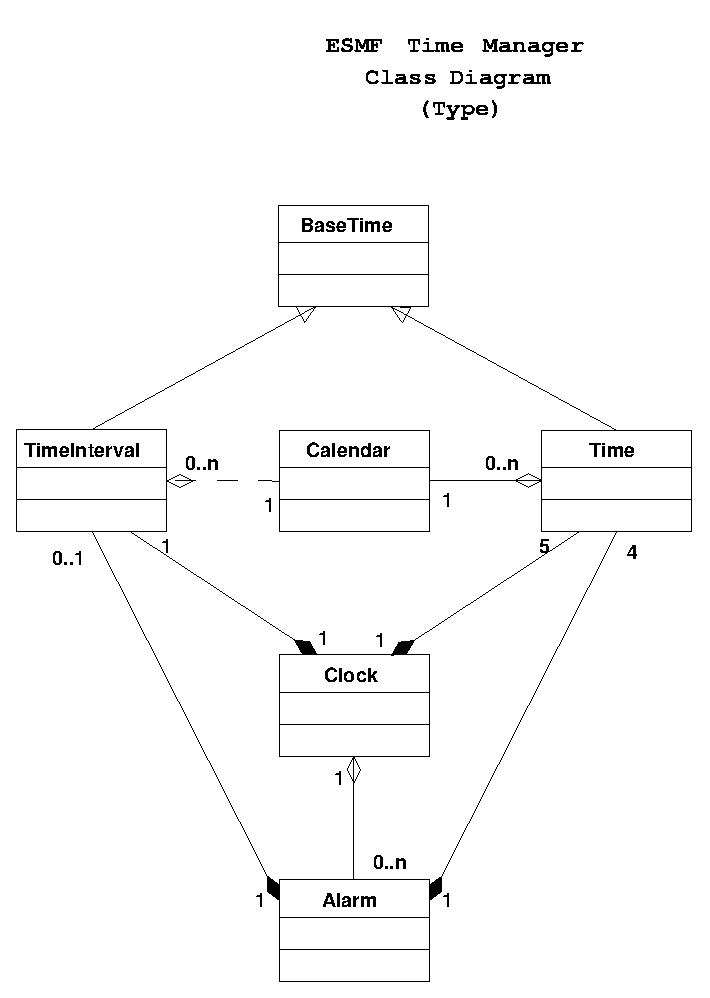
\includegraphics{TimeMgrClass.EPS}
   
Figure 1.  ESMF Time Manager Class Diagram
   
\end{center}
